\subsection{Experimental Methodology and Results}
In the following paragraphs, we report the methodology and results of our experiments.

\subsubsection{RQ1. Mono-objective SBSE Validation}
\paragraph{Method}

To answer the first research question RQ1, we conduct a mono-objective search for compiler optimizations exploration in order to evaluate the non-functional properties of optimized code. Thus, we use to generate optimization sequences using three search-based techniques (RS, GA and NS) and compare their performance results to standard GCC optimization levels (O1, O2, O3 and Ofast). 
In this experiment, we choose to optimize for execution time (S), memory usage (MR) and CPU consumption (CR). Each non-functional property is improved separately and independently of other metrics. Of course, other properties can be also optimized (e.g., code size, compilation time, etc.), but in this experiment, we focus only on these properties.

\begin{figure}[h]
	\centering
	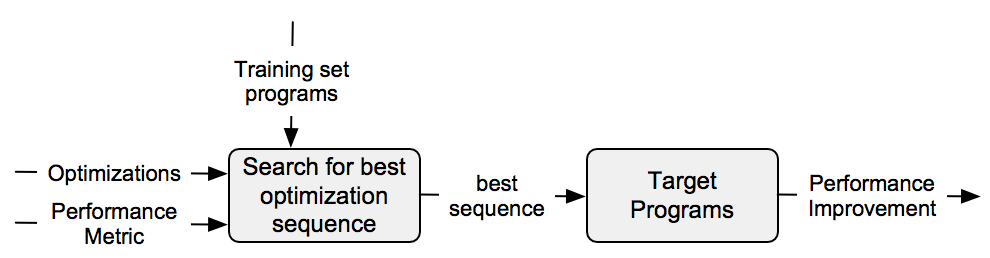
\includegraphics[width=1.\linewidth]{Ressources/sensitivity.png}
	\caption{Evaluation method to answer RQ1 and RQ2}
\end{figure}
As it is shown on the left-hand side of figure 5, given a list of optimizations and a performance objective, we use NOTICE to search for best optimization sequence across a set of input programs that we call \textit{"the training set"}. Thus, we generate a set of random Csmith programs \textit{"the training set"} (10 programs) and apply generated sequences to these programs. Therefore, the code quality metric, in this setting, is equal to the average performance improvement (S, MR or CR) and that, for all programs under test. 

%while p
%the goal of this initial experiment is to: (1) evaluate the effectiveness of our component-based infrastructure to extract non-functional properties such as memory and CPU consumptions; (2) evaluate the performance of our proposed diversity-based exploration of optimization sequences (NS) to GA and RS; and finally (3) find the optimal solution relative to the input training set.

%The goal of this experiment is to show that NOTICE is able to generate 





\paragraph{Results}



%\iffalse
\begin{table}[h]
	\centering
	\caption{Mono-objective optimization results}
	\label{my-label}
	\begin{tabular}{|l|l|l|l|l|l|l|c|}
		\hline
		& \textbf{O1}                    & \textbf{O2}                    & \textbf{O3}                    & \textbf{Ofast}                 & \textbf{RS}                    & \textbf{GA}                    & 
		\textbf{NS} \\
		\hhline{|=|=|=|=|=|=|=|=|}
		S  &  1.051 & 1.107  & 1.107  & 1.103  & 1.121  &  1.143 &  1.365  \\ \hline
		MR(\%) & 4.8  & -8.4  &  4.2 & 6.1  &  10.70 & 15.2  &  15.6  \\ \hline
		CR(\%) & -1.3  & -5  & 3.4  & -5  &  18.2 & 22.2  &  23.5  \\ \hline
	\end{tabular}
\end{table}
%\fi
%-NS better than 3 algos\\
%-conflicting results for standard levels
%The goal of this first experiment is to compare the performance improvement of novelty-based generated sequences to standard GCC optimizations and to RS and GA.  
Table 3 reports the comparison results of 3 non-functional properties CR, MR and S. Results describe the percentage improvement of MR and CR over the baseline, which is the O0 version. The speedup is also calculated over the baseline. At the first glance, we can clearly see that all search-based meta-heuristics outperform standard GCC levels with minimum improvement of 10\% for memory usage and 18\% for CPU time when applying RS. 
Our proposed NS approach has the best improvement results for 3 metrics with 1.365 of speedup, 15.6\% of memory reduction and 23.5\% of CPU time reduction. NS is clearly better than GA in terms of speedup. However, for MR and CR, NS is slightly better than GA with 0.4\% improvement for MR and 1.3\% for CR. RS has the lowest optimization performance but is still better than standard levels.
We remark as well that applying standard optimizations has an impact on the execution time with a speedup of 1.107 for O2 and O3. Ofast has the same impact as O2 and O3 for the execution time. However, the impact of GCC levels on resource consumption is not always efficient. O2, for example, increases resource consumption compared to O0 (-8.4\% for MR and -5\% for CR).
%Thus, NOTICE can clearly provide an alternative to catch most relevant optimization sequence regarding resource consumptions.
 	
%This agrees to the idea that standard optimizations mdoes not produce always
%the same impact results on resource consumption and may be highly dependent on the benchmark and the source code they have been tested on.
 %Using O2, we find that the memory consumption has increased by almost 8.4\% compared to the baseline. Same findings for CR when applying O1, O2 and Ofast. 



\noindent\fbox{\parbox{\linewidth-2\fboxrule-2\fboxsep}{
		\textbf{Key findings for RQ1.} \\
-- Best discovered optimization sequences using mono-objective search techniques always provide better results than standard GCC optimization levels.\\
-- Novelty Search is a good candidate to improve code in terms of non-functional properties since it able to discover optimization combinations that outperform RS and NS  }}
\subsubsection{RQ2. Sensitivity}
\paragraph{Method}
Another interesting experiment is to test the sensitivity of \textit{"training set"} programs to compiler optimizations and evaluate the general applicability of best optimal optimization sets previously discovered in RQ1 (i.e., sequences generated using NS relative to each non-functional property). To this end, we apply best discovered optimizations to new unseen Csmith (100 new random programs) and we compare then, the performance improvements (see right-hand side of figure 5). The idea of this experiment is to test whether new Csmith programs are more sensitive to previously discovered optimizations or not. If so, this will be useful for compiler users and researchers to use NOTICE in order to build general optimization sequences from their representative training set programs.

\paragraph{Results}
results

\noindent\fbox{\parbox{\linewidth-2\fboxrule-2\fboxsep}{
		\textbf{Key findings for RQ2.} \\
		blabla }}
\subsubsection{RQ3. Impact of optimizations on resource consumption}
\paragraph{Method}
In this experiment, we use NOTICE to provide an understanding of optimizations behavior, in terms of resource consumption, when trying to optimize for execution time. Thus, we choose one instance of obtained results in RQ1 related to the best speedup improvement (i.e., results obtained in line 1 of table 3) and we study the impact of performance improvement on memory and CPU consumption. We also compare resource consumption data to standard GCC levels as they ware presented in Table 3. Improvements are always calculated over the non-optimized version. The idea of this experiment is to: (1) prove, or not, the usefulness of involving resource metrics as key objectives for performance improvement; (2) the need, or not, of multi-objective search strategy to handle both resource usage and performance metrics.

%In this experiment, we apply standard optimizations and different mono-objective heuristics individually to 5 Cbench programs and use NOTICE to profile applications in terms of resource usage.  

%To answer RQ3, we choose one instance of obtained results in RQ1 related to the best improvement in terms of execution time (i.e., where NS had the best speedup) and we study the impact of performance improvement on memory and CPU consumption. 
%Following again a mono-objective approach, we try in this experiment to maximize the speedup \textit{S} per-benchmark and study, at the same time, the impact of speedup \textit{S} on resource consumption namely memory footprint and CPU usage. 
%In this experiment, we apply standard optimizations and different mono-objective heuristics individually to 5 Cbench programs and use NOTICE to profile applications in terms of resource usage.   
%The goal of this experiment is to: (1) use NOTICE infrastructure to provide an understanding of optimizations behavior, in terms of resource consumption, when trying to optimize for execution time; (2) prove the usefulness of resource consumption reduction as a key objective for performance improvement.

\paragraph{Results}

%\begin{figure}[h]
%	\centering
%	\includegraphics[width=1.\linewidth]{Ressources/infra_novelty_stat2.png}
%	\caption{Evaluating the speedup after applying standard optimization options compared to best generated optimization using NS}
%\end{figure}
results

\begin{figure}[h]
	\centering
	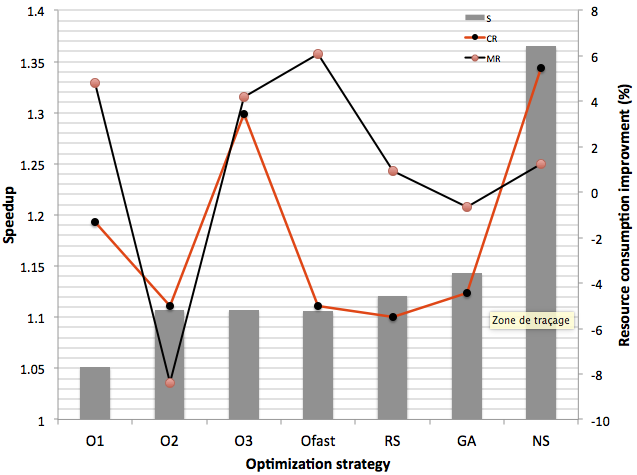
\includegraphics[width=1.\linewidth]{Ressources/rq3.png}
	\caption{Resource consumption when trying to optimize for time}
\end{figure}

\noindent\fbox{\parbox{\linewidth-2\fboxrule-2\fboxsep}{
		\textbf{Key findings for RQ3.} \\
		blabla }}
\subsubsection{RQ4. Trade-offs between non-functional properties}
\paragraph{Method}

Finally, to answer RQ4, we use NOTICE to find trade-offs between non-functional properties. In this experiment, we choose to focus on the trade-off \textit{$<$ExecutionTime--MemoryUsage$>$}. We report the comparison results of our NS adaptation for optimizations generation to the current state-of-the-art multi-objective approaches namely NSGA-II and RS. 
  
Sequences evaluation is done across 5 Cbench programs as it is conducted in RQ1.
We evaluate the quality of the obtained Pareto optimal optimization levels, both qualitatively by visual inspection of the Pareto frontiers, and quantitatively by using the HV metric.

%Two tradeoffs are investigated in this section; $<$execution time--memory usage$>$ and $<$execution time--CPU usage$>$.


\paragraph{Results}
RESULTS

\noindent\fbox{\parbox{\linewidth-2\fboxrule-2\fboxsep}{
		\textbf{Key findings for RQ4.} \\
		blabla }}
\subsection{Discussions}
For RQ1, experiments take about 21 days to run all algorithms. These optimization times might seem long. However, it should be noted that this search can be conducted only once, since in RQ2, we show that best optimizations can be used with unseen programs of the same category as the training set, used to generate optimizations. This has to be proved with other case studies. As an alternative, it would be great to test model-based code generators. Code generators apply to same rules to generate new software programs. Thus, we can use NOTICE to define general-purpose optimizations from a set of generated code artifacts. 
Multi-objective search as conducted in RQ4, takes about 7 days, which we believe is acceptable for practical use. Nevertheless, speeding up the search speed
may be an interesting feature for future research.



%speeding up the search process may be an interesting avenue for future research.
\subsection{Threats to Validity}
Any automated approach has limitations. We resume, in the following paragraphs, external and internal threats that can be raised:
 
\textit{External validity} refers to the generalizability of our findings. In this study, we perform experiments on random programs using Csmith and we use iterative compilation techniques to produce best optimization sequences. We believe that the use of Csmith programs as input programs is very relevant because compilers have been widely tested across Csmith programs~\cite{chen2016empirical,yang2011finding}. Csmith programs has been used only for functional testing, but not for non-functional testing. However, we cannot assert that the best discovered set of optimizations can be generalized to industrial applications since optimizations are highly dependent on input programs and on the target architecture. In fact, experiments conducted on RQ1 and RQ2 should be replicated to other case studies to confirm our findings; and build general optimization sequences from other representative training set programs chosen by compilers users.
Moreover, we build NOTICE to handle only optimizations performed by GCC versions, we did not investigate optimizations performed by other commonly used compilers, such as Clang or LLVM. In future work, we plan to provide more advanced version of NOTICE with multi-compiler evaluation.

\textit{Internal validity} is concerned with the causal relationship between the treatment and the outcome. Meta-heuristic algorithms are stochastic optimizers, they can provide different results for the same problem instance from one run to another. Are we providing a statistically sound method? or it is just a random result. Due to time constraints, we run all experiments only once. Following the state-of-the-art approaches in iterative compilation, previous research efforts~\cite{hoste2008cole,martinez2014multi} did not provide statistical tests to prove the effectiveness of their approaches. This is because experiments are time consuming. However, we can deal with these internal threats to validity by performing at least 5 independent simulation runs for each problem instance. 
 
 
\iffalse
\begin{table}[]
	\centering
	\caption{My caption}
	\label{my-label}
	\begin{tabular}{@{}|l|c|c|c|c|c|c|c|c|c|c|c|c|c|c|c|c|c|c|c|c|@{}}
		\toprule
		\multirow{2}{*}{} & \multicolumn{2}{c|}{CB1} & \multicolumn{2}{c|}{CB2} & \multicolumn{2}{c|}{CB3} & \multicolumn{2}{c|}{CB4} & \multicolumn{2}{c|}{CB5} & \multicolumn{2}{c|}{CS1} & \multicolumn{2}{c|}{CS2} & \multicolumn{2}{c|}{CS3} & \multicolumn{2}{c|}{CS4} & \multicolumn{2}{c|}{CS5} \\ \cmidrule(l){2-21} 
		& Ox & Best & Ox & Best & Ox & Best & Ox & Best & Ox & Best & Ox & Best & Ox & Best & Ox & Best & Ox & Best & Ox & Best \\ \midrule
		Execution Speedup & \begin{tabular}[c]{@{}c@{}}4\%\\ (O3)\end{tabular} &  &  &  &  &  &  &  &  &  &  &  &  &  &  &  &  &  &  &  \\ \midrule
		Memory & \begin{tabular}[c]{@{}c@{}}4\%\\ (O3)\end{tabular} &  &  &  &  &  &  &  &  &  &  &  &  &  &  &  &  &  &  &  \\ \midrule
		CPU & \begin{tabular}[c]{@{}c@{}}4\%\\ (O3)\end{tabular} &  &  &  &  &  &  &  &  &  &  &  &  &  &  &  &  &  &  &  \\ \midrule
		Compilation Speedup &  &  &  &  &  &  &  &  &  &  &  &  &  &  &  &  &  &  &  &  \\ \midrule
		Code Size &  &  &  &  &  &  &  &  &  &  &  &  &  &  &  &  &  &  &  &  \\ \bottomrule
	\end{tabular}
\end{table}
\fi


 

